% =============================================================================
% P3 --- version revisada: criterio de presencia por "hueco de separacion".
% Sustituye integramente la seccion P3. Figura nueva: presencia_criterio_k.png
% (generada por scripts/criterio_k_presencia.py).
% =============================================================================
\section{P3 --- ¿Puede el sistema confirmar operativamente la presencia de un dron?}
\label{sec:bloque_presencia}

\subsection{Planteamiento del experimento}
\label{sec:p3_planteamiento}

El recall de caja del \SI{39}{\percent} del experimento P2 mide la capacidad de localizar \emph{cada ráfaga individual} con precisión geométrica. Sin embargo, esa no es la pregunta operativa de un sistema de vigilancia, que no es «¿cuántas ráfagas detecta el modelo?», sino «\emph{dado un espectrograma de \SI{0.1}{\second}, indica el sistema correctamente si hay un dron presente?}».

Para responderla se define un \textbf{clasificador de presencia} muy simple: se cuentan todas las cajas de clase \emph{drone} que el detector emite sobre la ventana --- sin filtrar por confianza, es decir, todas las detecciones candidatas --- y se declara la ventana positiva si ese número alcanza al menos un umbral~$K$. La clave del experimento es determinar el valor de~$K$ con un criterio objetivo, no arbitrario.

\paragraph{Criterio para elegir $K$: el hueco de separación.}
El valor adecuado de~$K$ se obtiene observando dos magnitudes medidas sobre el conjunto de prueba:

\begin{itemize}
  \item el \textbf{suelo de falsos}: el número máximo de cajas \emph{drone} que el detector emite en una ventana que \emph{no} contiene dron;
  \item el \textbf{suelo de verdaderos}: el número mínimo de cajas \emph{drone} que emite en una ventana que \emph{sí} contiene dron.
\end{itemize}

Si existe un hueco entre ambos --- es decir, si el peor caso de una ventana con dron supera al peor caso de una ventana sin dron --- cualquier $K$ situado en ese hueco separa las dos clases sin error. El $K$ recomendado es el punto medio del hueco, que maximiza el margen frente a los dos tipos de error simultáneamente.

\subsection{Resultados}
\label{sec:p3_resultados}

La \cref{fig:presencia_criterio_k}(a) muestra la distribución del número de cajas \emph{drone} por ventana para las \num{300}~imágenes con dron y las \num{300}~sin dron del conjunto de prueba. Las dos poblaciones están completamente separadas: las ventanas sin dron acumulan como máximo \textbf{3}~cajas \emph{drone} espurias, mientras que la ventana con dron más pobre presenta \textbf{11}~cajas. Existe, por tanto, un hueco de separación limpio en el intervalo $(3, 11]$.

\begin{figure}[htbp]
    \centering
    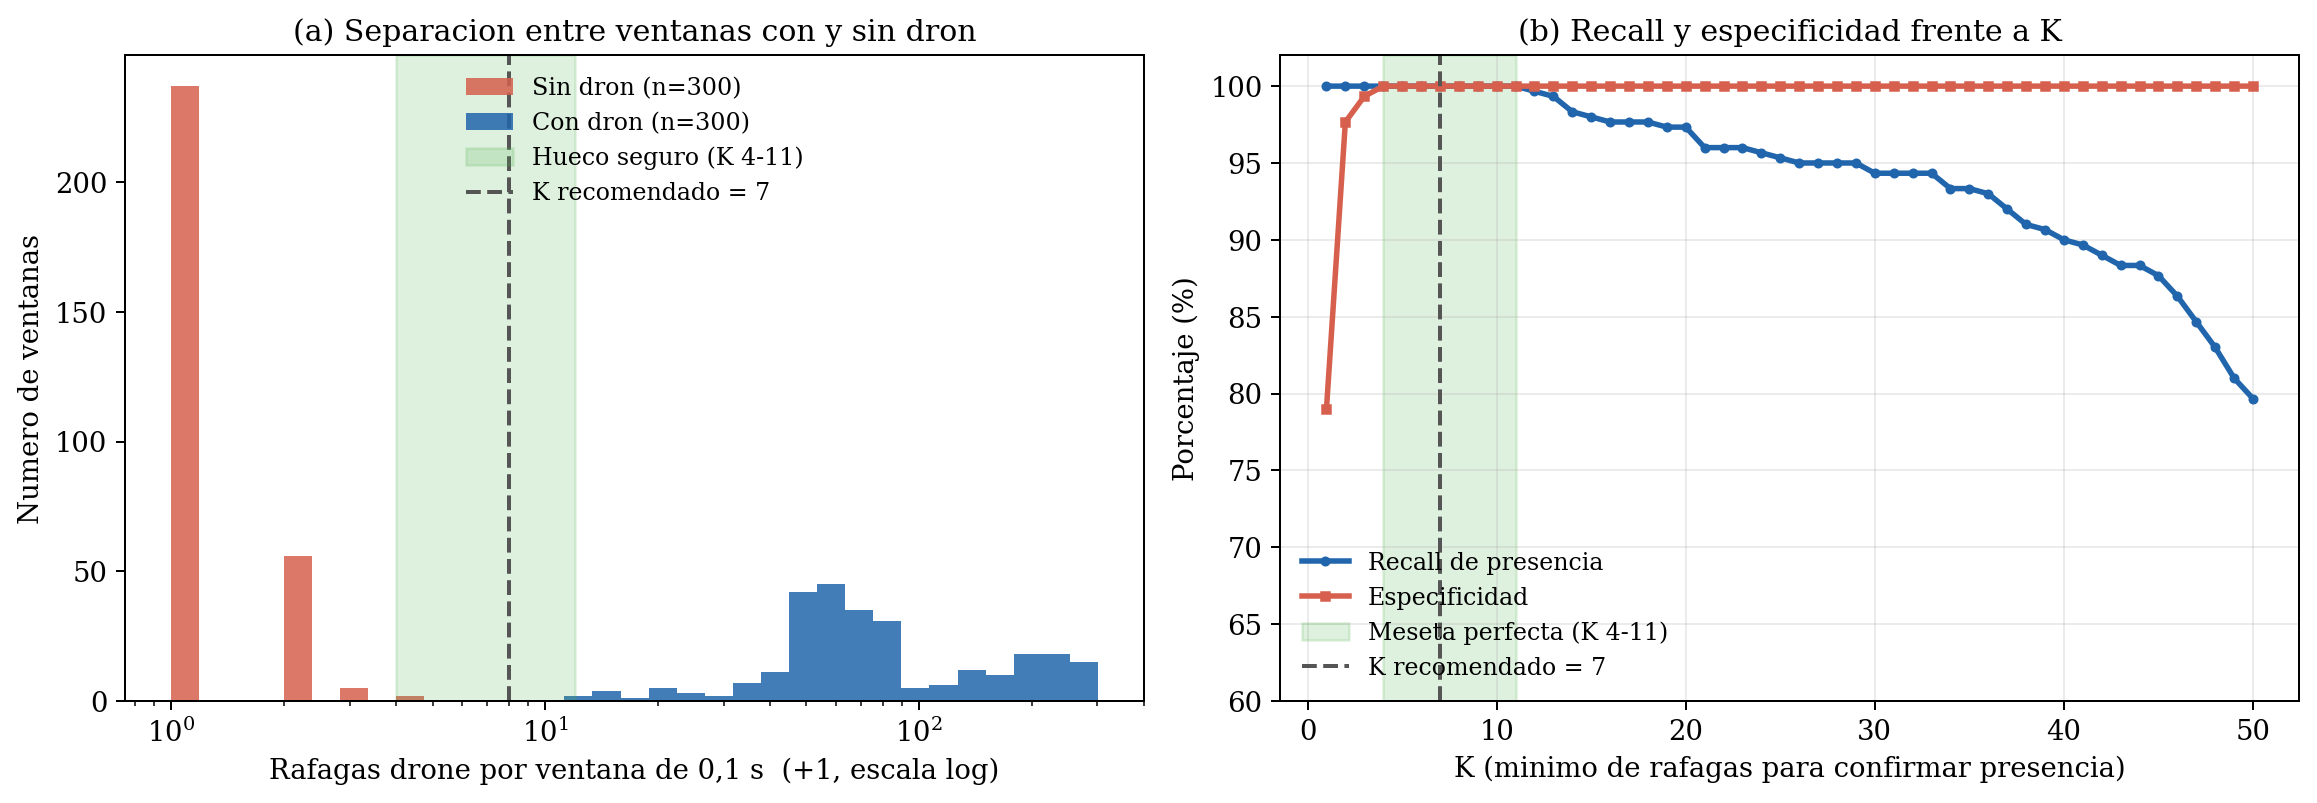
\includegraphics[width=\textwidth]{figuras/resultados/presencia_criterio_k.png}
    \caption{Determinación del criterio de presencia. (a) Distribución del número de ráfagas \emph{drone} detectadas por ventana de \SI{0.1}{\second} (escala logarítmica) para las ventanas con dron (azul) y sin dron (rojo). Las dos poblaciones no se solapan: existe un hueco de separación (banda verde) entre el suelo de falsos (\num{3}~cajas) y el suelo de verdaderos (\num{11}~cajas). (b) Recall de presencia y especificidad en función de~$K$. Para todo $K\in[4,11]$ (meseta verde) ambas métricas valen \SI{100}{\percent}. La línea discontinua marca el valor recomendado $K=7$, punto medio del hueco.}
    \label{fig:presencia_criterio_k}
\end{figure}

La \cref{fig:presencia_criterio_k}(b) confirma la consecuencia directa de ese hueco: al barrer $K$ desde 1 hasta 50, el recall de presencia y la especificidad alcanzan ambos el \SI{100}{\percent} en toda la meseta $K\in[4,11]$. La \cref{tab:presencia_sweep_k} detalla el barrido en el entorno relevante.

\begin{table}[htbp]
\centering
\caption{Métricas del clasificador de presencia en función de~$K$ (conteo de todas las cajas \emph{drone} candidatas), sobre las \num{600}~imágenes de prueba (\num{300} con dron, \num{300} sin dron).}
\label{tab:presencia_sweep_k}
\begin{tabular}{ccccc}
\toprule
\textbf{$K$} & \textbf{Recall (\%)} & \textbf{Especificidad (\%)} & \textbf{Precisión (\%)} & \textbf{F1} \\
\midrule
1  & 100,0 & 79,0  & 82,6  & 0,905 \\
2  & 100,0 & 97,7  & 97,7  & 0,988 \\
3  & 100,0 & 99,3  & 99,3  & 0,997 \\
4  & 100,0 & 100,0 & 100,0 & 1,000 \\
5  & 100,0 & 100,0 & 100,0 & 1,000 \\
6  & 100,0 & 100,0 & 100,0 & 1,000 \\
\textbf{7}  & \textbf{100,0} & \textbf{100,0} & \textbf{100,0} & \textbf{1,000} \\
8  & 100,0 & 100,0 & 100,0 & 1,000 \\
9  & 100,0 & 100,0 & 100,0 & 1,000 \\
10 & 100,0 & 100,0 & 100,0 & 1,000 \\
11 & 100,0 & 100,0 & 100,0 & 1,000 \\
12 & 99,7  & 100,0 & 100,0 & 0,998 \\
\bottomrule
\end{tabular}
\end{table}

En el punto de operación recomendado $K=7$, el sistema clasifica correctamente las \num{600}~imágenes del conjunto de prueba: \num{300}~verdaderos positivos, \num{300}~verdaderos negativos, \textbf{cero} falsos positivos y \textbf{cero} falsos negativos (recall, especificidad, precisión y F1 iguales a \num{1,000}). El desglose por captura es igualmente nítido: las dos capturas con dron --- a \SI{10}{\meter} con WiFi saturado (L3) y a \SI{5}{\meter} con WiFi limpio (L1) --- se confirman en el \SI{100}{\percent} de sus ventanas, y las dos capturas de interferencia pura se rechazan en el \SI{100}{\percent}, sin una sola falsa alarma.

\subsection{Discusión}
\label{sec:p3_discusion}

El resultado de P3 es la confirmación operativa del sistema: con el criterio de presencia y $K=7$, la decisión a nivel de ventana es perfecta sobre el conjunto de prueba, pese a que el recall de caja individual del detector es solo del \SI{39}{\percent}.

\paragraph{Por qué un recall de caja del 39\,\% produce una decisión perfecta.}
La explicación está en la \cref{fig:presencia_criterio_k}(a): una ventana con dron contiene decenas de ráfagas OcuSync (mediana de \num{72}~cajas detectadas, mínimo de \num{11}), consecuencia directa del diseño FHSS del protocolo, que salta de canal decenas de veces por cada \SI{0.1}{\second}. Aunque el detector falle la mayoría de las ráfagas a nivel individual, le basta con acertar unas pocas de las muchas que ofrece cada imagen. El clasificador de presencia actúa como un agregador que convierte múltiples detecciones débiles en una decisión binaria robusta: la redundancia temporal del protocolo transforma un recall de caja modesto en una separación de presencia total.

\paragraph{Por qué $K=7$.}
El valor $K=7$ es el punto medio del hueco $(3, 11]$: deja un margen de \num{4}~ráfagas por encima del peor caso de una ventana sin dron y de \num{4}~ráfagas por debajo de la ventana con dron más pobre. Cualquier $K$ entre \num{4} y \num{11} produce el mismo resultado perfecto sobre el test; la elección del punto medio simplemente maximiza la tolerancia a que, en condiciones distintas, suba el suelo de falsos o baje el de verdaderos. Frente a un criterio de $K$ bajo pegado al suelo de ruido, $K=7$ no sacrifica ningún dron y elimina por completo el riesgo de falsas alarmas por detecciones espurias aisladas.

\paragraph{Alcance y limitaciones.}
La separación perfecta debe interpretarse en el contexto del conjunto de prueba: dos capturas con dron y dos de interferencia, en el entorno interior controlado del dataset~v3 (\cref{cap:implementacion}). El hueco $(3, 11]$ está estimado sobre esas capturas; en un despliegue con mayor diversidad de distancias, niveles de interferencia y entornos, es esperable que el suelo de falsos suba y el de verdaderos baje, estrechando el hueco. El resultado relevante no es el valor numérico concreto $K=7$, sino el \emph{método}: medir ambos suelos sobre datos representativos y situar~$K$ en el hueco resultante. La validación de este criterio sobre un conjunto más variado (dataset~v4, \cref{cap:conclusiones}) queda como trabajo futuro.
